\documentclass[10pt]{article}
\usepackage[margin=2.2cm]{geometry}
\usepackage{booktabs,longtable,graphicx,array,xcolor,framed}
\usepackage[hidelinks]{hyperref}
\setlength{\tabcolsep}{4pt}
\title{Tuning report: tropical / MaxSubsetSum}
\date{2026-10-22T19:16:57}
\begin{document}
\maketitle

\section{Decision}
Approving freezes
\texttt{fishr.lambda} $=$ 100 into every cell of the grid (frozen hash \texttt{a7b38650bd58}).
The experiment YAML has
\texttt{fishr.lambda} $=$ 1000 for this campaign.
\texttt{frozen.yaml} is currently unapproved with \{'fishr.lambda': 100.0\}.

\paragraph{Selection rule.} The candidate with the lowest mean \texttt{id\_val\_loss} wins, averaged over 6 cell(s) and 2 tuning seed(s) each (global seed 1000, disjoint from the grid's 0), across 4 candidates. A candidate with a missing or diverged run is not eligible.

\begin{framed}
\noindent\textbf{Verdict: \textcolor{orange!85!black}{REVIEW}}
\begin{itemize}\setlength\itemsep{0pt}
\item \textbf{review}: the candidate means differ by less than 0.1\%: the metric barely responds to the knob
\item \textbf{review}: the winner is not distinguishable from fishr.lambda=10: the paired gap's 95\% CI is [-1.74e-08, 3.55e-06]
\item \textbf{review}: fishr.lambda=10: fishr.lambda * fishr\_penalty\_final is 4.8e-05 of id\_val\_loss (median over runs); the term barely enters the loss
\item \textbf{review}: fishr.lambda=100: fishr.lambda * fishr\_penalty\_final is 0.00048 of id\_val\_loss (median over runs); the term barely enters the loss
\item \textbf{review}: fishr.lambda=1000: fishr.lambda * fishr\_penalty\_final is 0.0048 of id\_val\_loss (median over runs); the term barely enters the loss
\item \textbf{review}: 12 of 12 winner runs reached their best id\_val\_loss at the last logged epoch: the search budget may be too short to rank candidates
\item \textbf{review}: 12 of 12 winner runs picked their last epoch (best\_epoch = 19): still improving when the search budget ran out, so candidates were ranked before converging
\item \textbf{info}: the search ran with optim.epochs=20; the grid runs with optim.epochs=100
\item \textbf{info}: devices: cuda:0
\end{itemize}
\end{framed}
\noindent\textbf{block}: do not approve; fix the search and re-run it. \textbf{review}: read the sections below before approving. \textbf{info}: context only.

\section{Search setup}
\begin{itemize}\setlength\itemsep{0pt}
\item \texttt{fishr.lambda} $\in \{$10, 100, 1000, 1e+04$\}$
\item Cells trained (\texttt{tune.only} \{'objective': 'fishr'\}):
\begin{itemize}\setlength\itemsep{0pt}
\item \texttt{model\_type=vanilla head=seq2seq objective=fishr}
\item \texttt{model\_type=vanilla head=pointer objective=fishr}
\item \texttt{model\_type=adaptive head=seq2seq objective=fishr}
\item \texttt{model\_type=adaptive head=pointer objective=fishr}
\item \texttt{model\_type=tropical head=seq2seq objective=fishr}
\item \texttt{model\_type=tropical head=pointer objective=fishr}
\end{itemize}
\item Search-only overrides (never frozen): \texttt{\{'optim': \{'epochs': 20\}\}}. The chosen value was ranked under this budget, not the grid's.
\end{itemize}

\section{Candidates}
\autoref{tab:candidates} ranks the candidates on \texttt{id\_val\_loss} (lower is better); \autoref{fig:sensitivity} plots them.
Candidates share seeds, so \autoref{tab:gaps} compares each with the winner run by run (same cell, same seed).

{\small
\begin{longtable}{rlrrrlrll}
\caption{Every candidate: rank, runs stored/expected, diverged, mean with 95\% bootstrap CI, SD and range over all its runs.}\label{tab:candidates}\\
\toprule
\# & \texttt{fishr.lambda} & runs & div. & mean & 95\% CI & SD & range & \\
\midrule
\endhead
2 & 10 & 12/12 & 0 & 0.03831 & [0.012, 0.0727] & 0.0589 & [$1.77\times10^{-4}$, 0.181] & \\
1 & 100 & 12/12 & 0 & 0.0383 & [0.012, 0.0737] & 0.0589 & [$1.77\times10^{-4}$, 0.181] & \textbf{selected}\\
3 & 1000 & 12/12 & 0 & 0.03831 & [0.00922, 0.0737] & 0.0589 & [$1.77\times10^{-4}$, 0.181] & \\
4 & 1e+04 & 12/12 & 0 & 0.03831 & [0.0114, 0.0736] & 0.059 & [$1.77\times10^{-4}$, 0.181] & \\
\bottomrule
\end{longtable}
}

{\small
\begin{longtable}{lrrlrrrl}
\caption{Each candidate minus the winner on the runs they share, signed so a positive gap is worse than the winner. Worse/better/equal count the runs; $p$ is a two-sided sign test.}\label{tab:gaps}\\
\toprule
candidate & $n$ & gap & 95\% CI & worse & better & equal & $p$\\
\midrule
\endhead
\texttt{fishr.lambda=10} & 12 & $1.392\times10^{-6}$ & [$-1.74\times10^{-8}$, $3.55\times10^{-6}$] & 2 & 10 & 0 & 0.0386\\
\texttt{fishr.lambda=1000} & 12 & $1.909\times10^{-6}$ & [$1.33\times10^{-7}$, $4.76\times10^{-6}$] & 12 & 0 & 0 & 0.0005\\
\texttt{fishr.lambda=10000} & 12 & $1.001\times10^{-5}$ & [$3.32\times10^{-8}$, $2.77\times10^{-5}$] & 11 & 1 & 0 & 0.0063\\
\bottomrule
\end{longtable}
}

\begin{figure}[htbp]
\centering
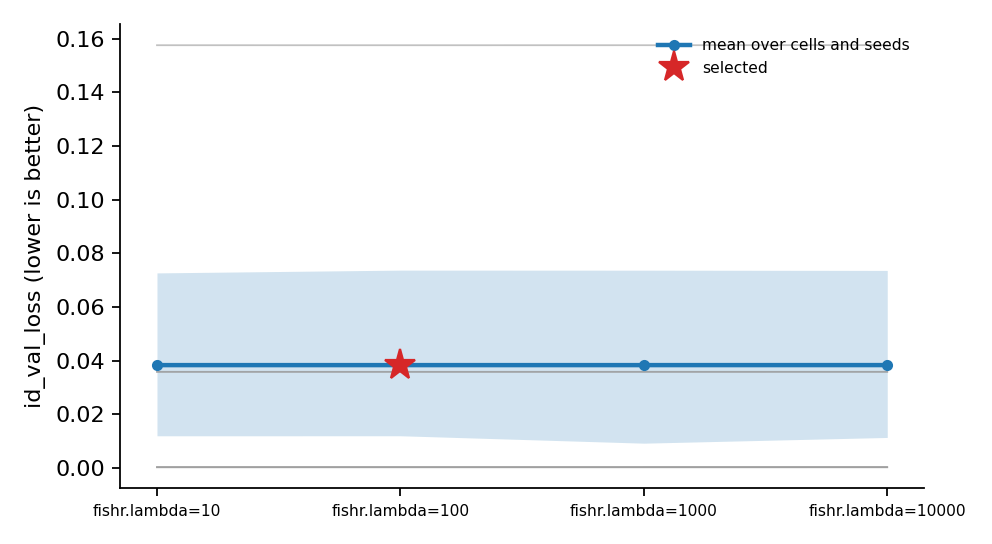
\includegraphics[width=\textwidth]{tune_sensitivity.png}
\caption{\texttt{id\_val\_loss} per candidate: the mean over every run with a 95\% bootstrap CI (blue), each cell's seed-mean (grey), the selected candidate (red star).}
\label{fig:sensitivity}
\end{figure}

\section{Per cell}
One value is frozen for every cell, chosen by the mean over cells. \autoref{fig:cells} shows whether the winner is best in each cell or is carried by a few of them.
\begin{figure}[htbp]
\centering
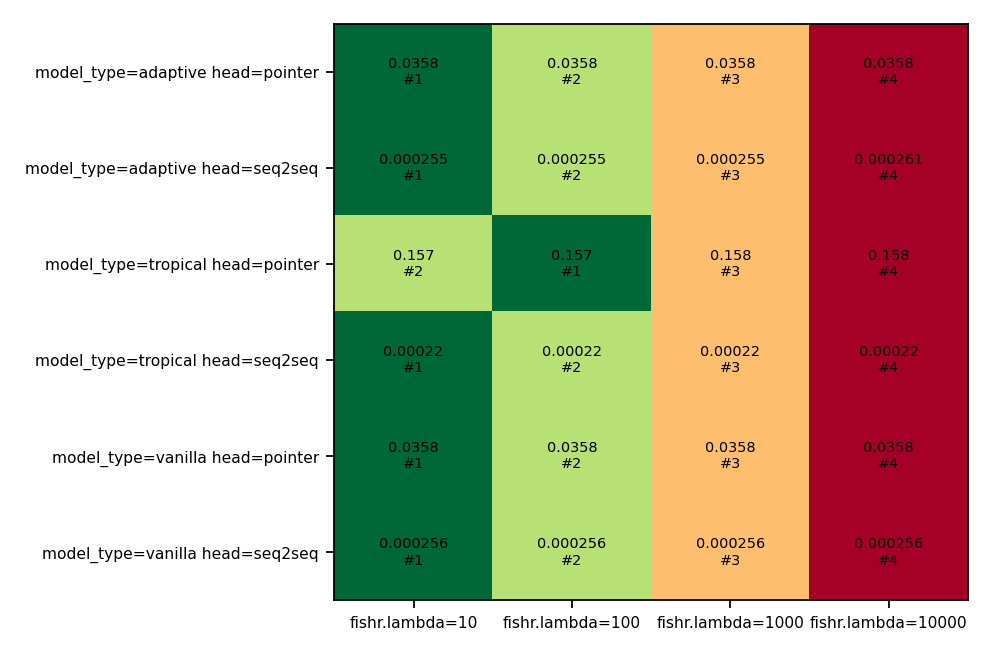
\includegraphics[width=\textwidth]{tune_cells.png}
\caption{Each cell's seed-mean \texttt{id\_val\_loss} per candidate, with its rank within the cell (\#1 is best; green is better).}
\label{fig:cells}
\end{figure}
{\small
\begin{longtable}{ll}
\caption{The best candidate in each cell.}\label{tab:cells}\\
\toprule
cell & best\\
\midrule
\endhead
\texttt{model\_type=adaptive head=pointer} & fishr.lambda=10\\
\texttt{model\_type=adaptive head=seq2seq} & fishr.lambda=10\\
\texttt{model\_type=tropical head=pointer} & fishr.lambda=100\\
\texttt{model\_type=tropical head=seq2seq} & fishr.lambda=10\\
\texttt{model\_type=vanilla head=pointer} & fishr.lambda=10\\
\texttt{model\_type=vanilla head=seq2seq} & fishr.lambda=10\\
\bottomrule
\end{longtable}
}

\section{Other training-distribution metrics}
Not used for selection; shown so a winner that trades them away is visible.
{\small
\begin{longtable}{lrrrr}
\caption{Mean of every other in-distribution metric per candidate.}\label{tab:open}\\
\toprule
candidate & \texttt{id\_f1} & \texttt{id\_exact} & \texttt{fishr\_penalty\_final} & \texttt{best\_epoch}\\
\midrule
\endhead
fishr.lambda=10 & 0.993 & 0.992 & $9.79\times10^{-7}$ & 19\\
\textbf{fishr.lambda=100} & 0.993 & 0.992 & $9.79\times10^{-7}$ & 19\\
fishr.lambda=1000 & 0.993 & 0.992 & $9.80\times10^{-7}$ & 19\\
fishr.lambda=10000 & 0.993 & 0.992 & $9.80\times10^{-7}$ & 19\\
\bottomrule
\end{longtable}
}

\section{Training curves}
The mean over every cell and seed of each candidate; the selected candidate in bold red.
\begin{figure}[htbp]
\centering
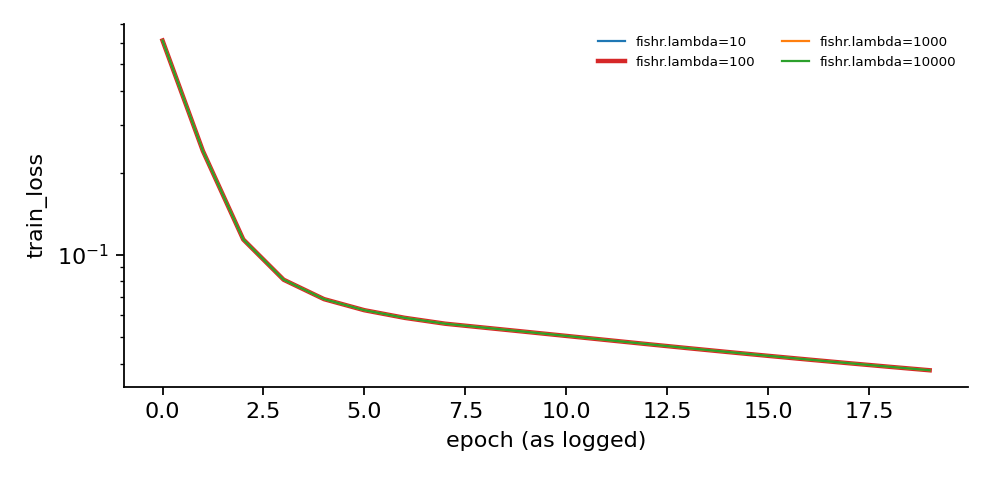
\includegraphics[width=\textwidth]{tune_curve_train_loss.png}
\caption{\texttt{train\_loss} per candidate.}
\label{fig:curve-train_loss}
\end{figure}
\begin{figure}[htbp]
\centering
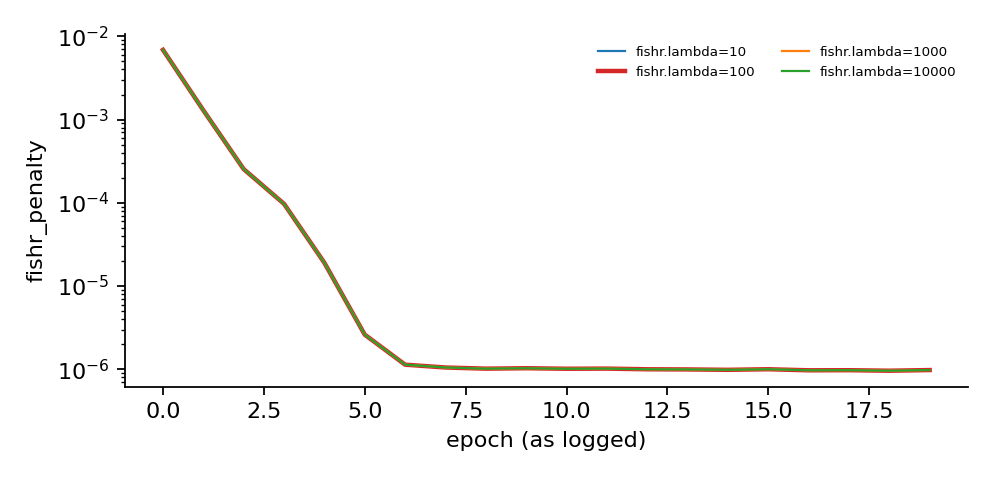
\includegraphics[width=\textwidth]{tune_curve_fishr_penalty.png}
\caption{\texttt{fishr\_penalty} per candidate.}
\label{fig:curve-fishr_penalty}
\end{figure}
\begin{figure}[htbp]
\centering
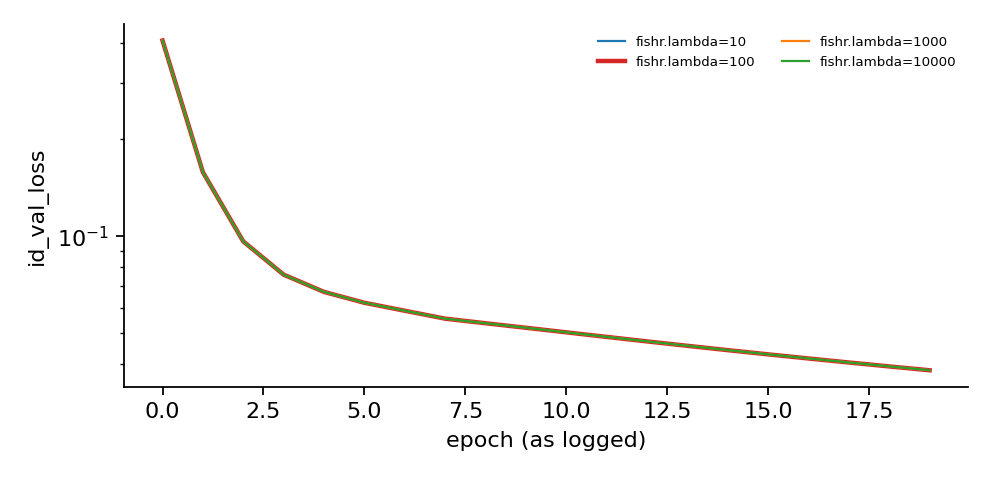
\includegraphics[width=\textwidth]{tune_curve_id_val_loss.png}
\caption{\texttt{id\_val\_loss} per candidate.}
\label{fig:curve-id_val_loss}
\end{figure}

\clearpage
\section{Provenance}
{\small
\begin{longtable}{llrrll}
\caption{Each candidate's runs: base hash, runs, total wall time, commits (+ marks a dirty tree), torch.}\label{tab:provenance}\\
\toprule
candidate & hash & runs & wall (s) & commit & torch\\
\midrule
\endhead
fishr.lambda=10 & \texttt{5f3ea28bbae6} & 12 & 3.56e+03 & \texttt{e5ccce8034} & 2.8.0+cu128\\
fishr.lambda=100 & \texttt{c7a3d04d3b06} & 12 & 3.6e+03 & \texttt{e5ccce8034} & 2.8.0+cu128\\
fishr.lambda=1000 & \texttt{84f145eac03b} & 12 & 3.6e+03 & \texttt{e5ccce8034} & 2.8.0+cu128\\
fishr.lambda=10000 & \texttt{254f24525e3f} & 12 & 3.6e+03 & \texttt{e5ccce8034} & 2.8.0+cu128\\
\bottomrule
\end{longtable}
}
\noindent Store: \texttt{campaigns/tropical/MaxSubsetSum/tune/results}.\\
Rebuild: \texttt{expkit tune-report --config configs/tropical.yaml --profile MaxSubsetSum}\\
Approve: \texttt{expkit approve --config configs/tropical.yaml --profile MaxSubsetSum}

\paragraph{The base the grid would run with.}
{\footnotesize
\begin{verbatim}
task:
  name: MaxSubsetSumDataset
  value_range:
  - -5
  - 5
  target_range: null
  weight_range: null
  adversarial_range:
  - 10
  - 30
  noise_prob: 0.0
data:
  train_lengths:
  - 4
  - 5
  - 6
  - 7
  - 8
  ood_lengths:
  - 12
  - 16
  - 64
  ood_value_range: null
  ood_noise_range: null
  ood_noise_prob: 0.5
  n_per_length: 20000
  n_eval_per_length: 2000
  curve_eval_limit: 256
model:
  d_model: 64
  n_heads: 2
  num_layers: 1
  dropout: 0.0
  tropical_impl: legacy
optim:
  lr: 0.0001
  epochs: 100
  batch_size: 100
  eval_batch_size: 256
fishr:
  lambda: 100.0
  ema: 0.95
  anneal_iters: 1500
  reset_optimizer: true
\end{verbatim}
}

\clearpage
\appendix
\section{Sealed: OOD and test metrics}
\textbf{Read this only after deciding.} These were recorded by the tuning runs but never consulted by the selection. Choosing a value because it looks better here would tune on the test distribution.
{\small
\begin{longtable}{lrrrrrrrrrrrr}
\caption{Mean of every OOD or test metric per candidate.}\label{tab:sealed}\\
\toprule
candidate & \rotatebox{70}{\texttt{ood\_len\_f1}} & \rotatebox{70}{\texttt{ood\_len\_exact}} & \rotatebox{70}{\texttt{ood\_val\_f1}} & \rotatebox{70}{\texttt{ood\_val\_exact}} & \rotatebox{70}{\texttt{ood\_noise\_f1}} & \rotatebox{70}{\texttt{ood\_noise\_exact}} & \rotatebox{70}{\texttt{ood\_len\_f1\_L12}} & \rotatebox{70}{\texttt{ood\_len\_exact\_L12}} & \rotatebox{70}{\texttt{ood\_len\_f1\_L16}} & \rotatebox{70}{\texttt{ood\_len\_exact\_L16}} & \rotatebox{70}{\texttt{ood\_len\_f1\_L64}} & \rotatebox{70}{\texttt{ood\_len\_exact\_L64}}\\
\midrule
\endhead
fishr.lambda=10 & 1 & 1 & 0.992 & 0.988 & 0.96 & 0.918 & 1 & 1 & 1 & 1 & 1 & 1\\
\textbf{fishr.lambda=100} & 1 & 1 & 0.992 & 0.988 & 0.96 & 0.918 & 1 & 1 & 1 & 1 & 1 & 1\\
fishr.lambda=1000 & 1 & 1 & 0.992 & 0.988 & 0.96 & 0.918 & 1 & 1 & 1 & 1 & 1 & 1\\
fishr.lambda=10000 & 1 & 1 & 0.992 & 0.988 & 0.96 & 0.918 & 1 & 1 & 1 & 1 & 1 & 1\\
\bottomrule
\end{longtable}
}
\end{document}